\chapter{Result And Discussion}
	\section{Model Evaluation}
	\begin{figure}[hbt!]
		\center{
			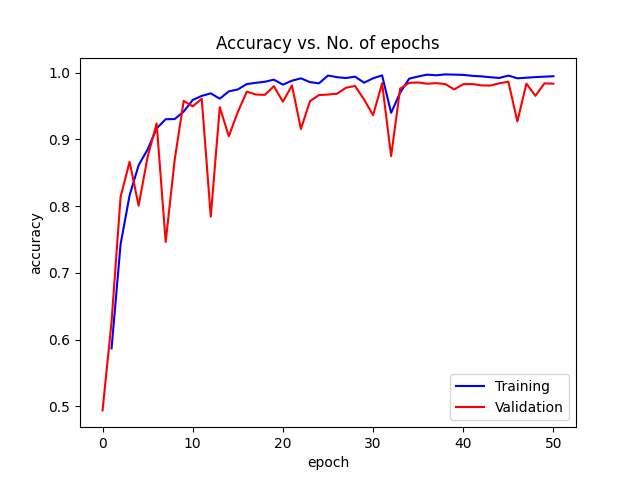
\includegraphics[width=0.7\textwidth]{./img/resnet9accuracy.png}
			\caption{Accuracy vs. No. of epochs }
		}
	\end{figure}
	\begin{figure}[hbt!]
		\center{
			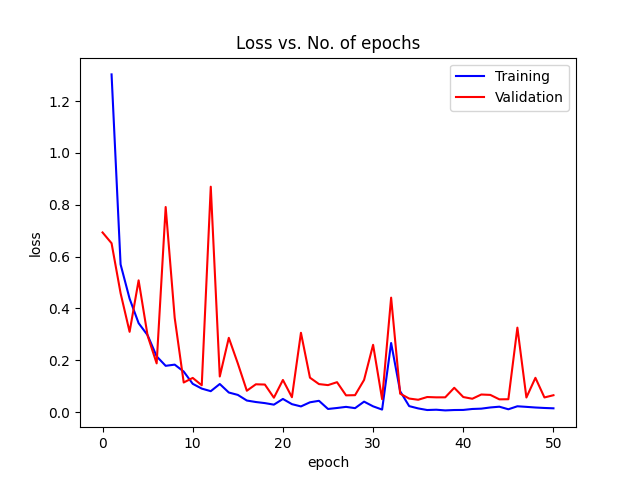
\includegraphics[width=0.7\textwidth]{./img/resnet9losses.png}
			\caption{Loss vs. No. of epochs}
		}
	\end{figure}

	\pagebreak
	\subsection*{Testing Results}
	We used the test dataset given on the DeepFake Detection Challenge\cite{jimaging8100263} to test our models performance.
	Testing dataset consist of 5000 fake images and 2000 real images.
	\vspace{1pt}
	\begin{figure}[hbt!]
		\center{
			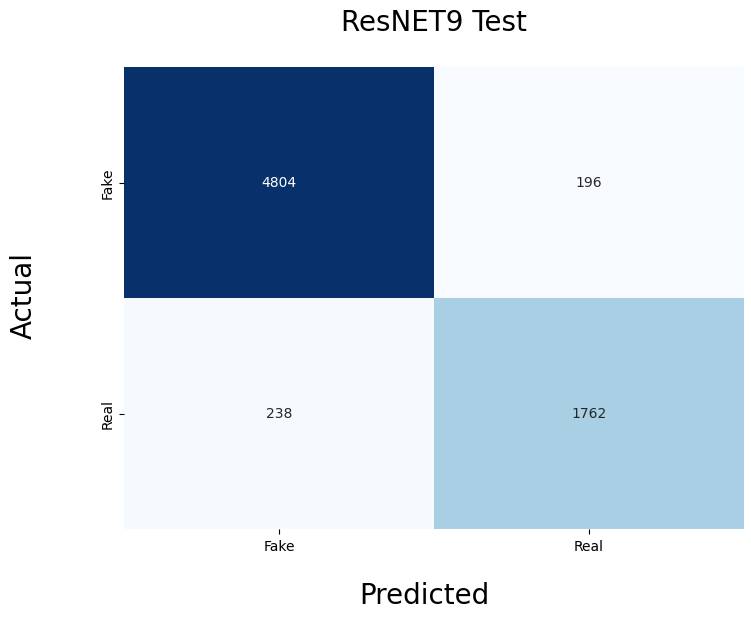
\includegraphics[width=1\textwidth]{./img/confusion_matrix.png}
			\caption{Confusion Matrix}
		}
	\end{figure}

	% \newpage
	\begin{enumerate}
		\item Accuracy
		\begin{equation}
				\text{Accuracy} = \frac{\text{TP} + \text{TN}}{\text{TP} + \text{TN} + \text{FP} + \text{FN}}
		\end{equation}
		\item Precision
		\begin{equation}
			% \begin{flalign}
				\text{Precision} = \frac{\text{TP}}{\text{TP} + \text{FP}}
			% \end{flalign}
		\end{equation}
		\item Recall
		\begin{equation}
			\text{Recall} = \frac{\text{TP}}{\text{TP} + \text{FN}}
		\end{equation}
		\item F1 Score
		\begin{equation}
			\text{F1 Score} = 2 \times \frac{\text{Precision} \times \text{Recall}}{\text{Precision} + \text{Recall}}
		\end{equation}

		where\\
		TP = True Positive,\\
		TN = True Negative,\\
		FP = False Positive,\\
		FN = False Negative
		\pagebreak
		\item Reciever Operating Characteristic (ROC) Curve
			\begin{figure}[hbt!]
				\center{
					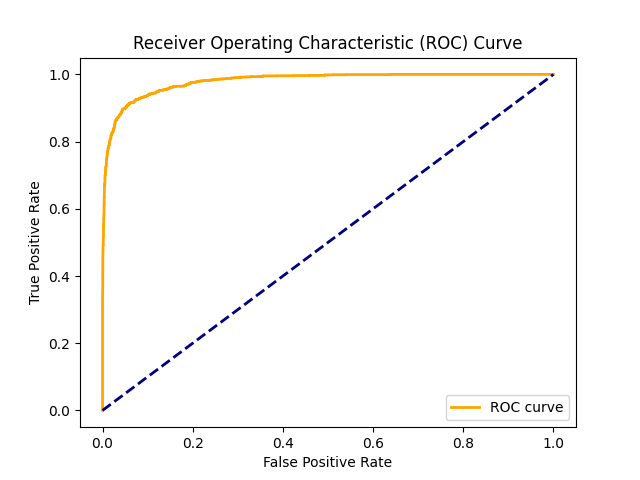
\includegraphics[width=1\textwidth]{./img/ROC.png}
					\caption{Reciever Operating Characteristic (ROC) Curve}
				}
			\end{figure}

			\textbf{Area Under ROC Curve = 0.9209}

\begin{table}[h!]
		\centering
		\begin{tabular}{lccccc}
		\multicolumn{6}{c}{\textbf{}} \\ 
		\multicolumn{6}{c}{\textbf{}} \\ 
		\textbf{} & \textbf{Accuracy} & \textbf{Precision} & \textbf{Recall} & \textbf{F1-score} & \textbf{Support} \\
		\textbf{Fake}  & 96.08\% & 0.952 & 0.960 & 0.955 & 5000 \\
		\textbf{Real} & 88.10\%  & 0.899 & 0.881 & 0.889 & 2000 \\
		\textbf{Macro Avg} & 92.09\% & 0.925 & 0.920 & 0.922 & 7000 \\
		\textbf{Weighted Avg} & 93.80\% & 0.936 & 0.938 & 0.937 &7000 \\ 
		\multicolumn{6}{c}{\textbf{}} \\
		\multicolumn{6}{c}{\textbf{}} \\
		\end{tabular}
		\caption{Performance Table}
		\end{table}
\end{enumerate}

\clearpage
\section{User Interface}

\begin{figure}[hbt!]
	\center{
		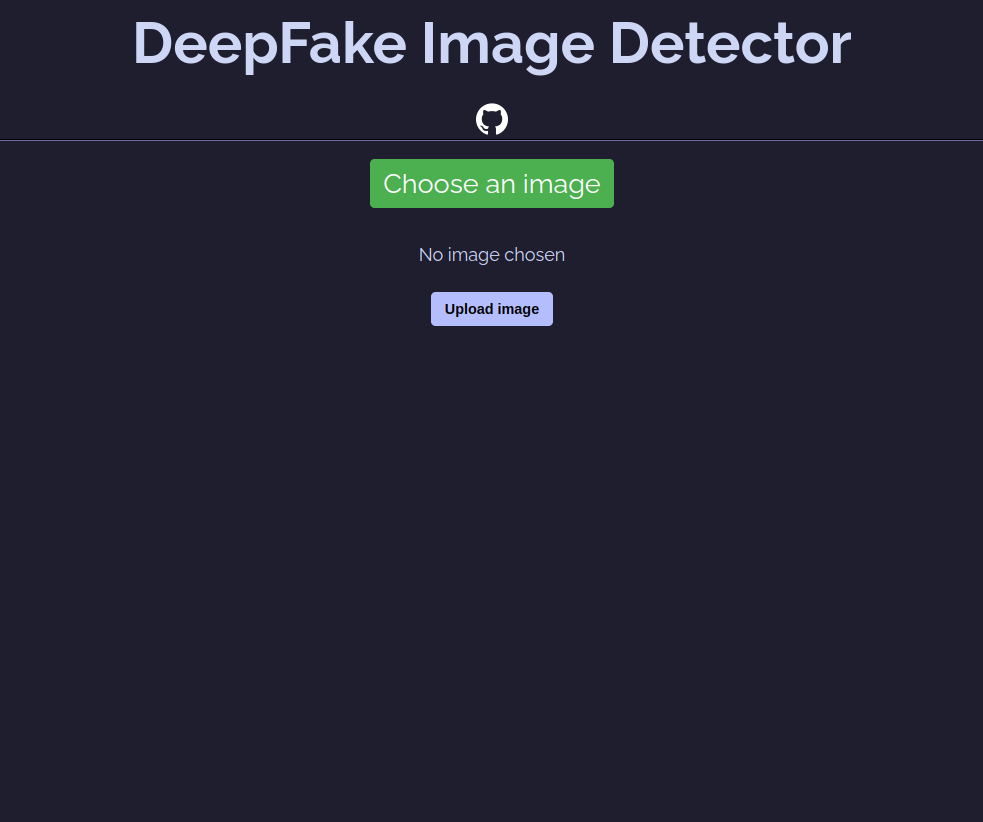
\includegraphics[width=0.66\textwidth]{./img/UI0.png}
		\caption{Home Page} }
\end{figure}

\begin{figure}[hbt!]
	\center{
		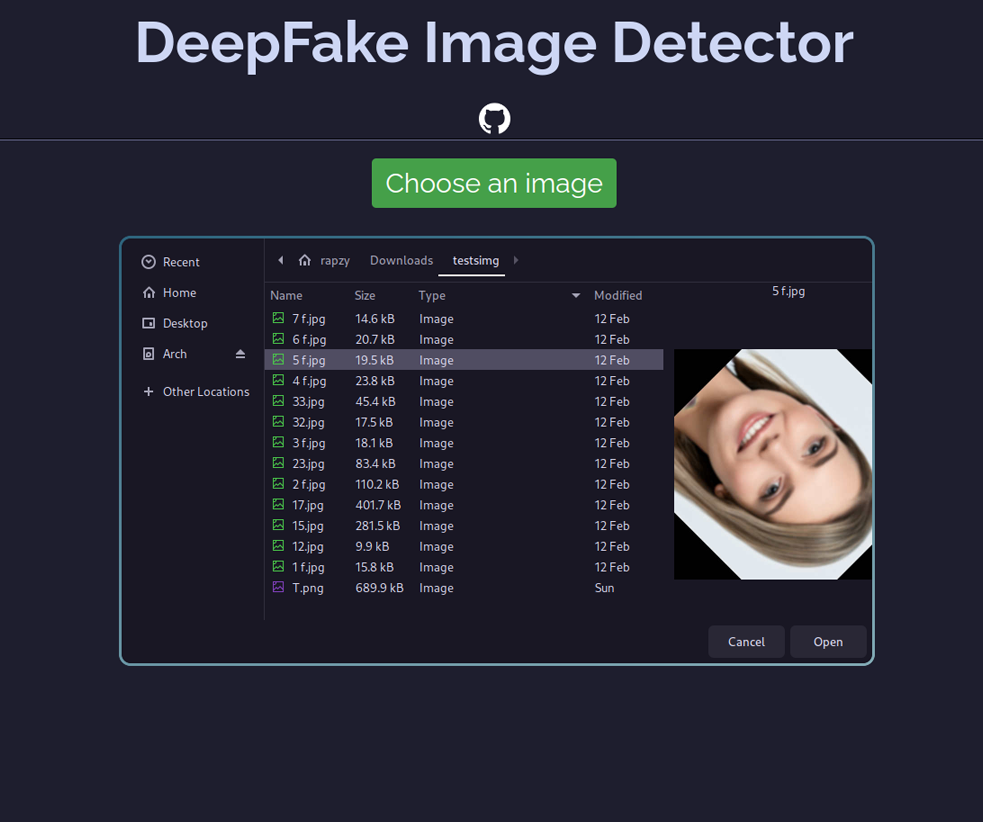
\includegraphics[width=0.66\textwidth]{./img/UI3.png}
		\caption{Browse Image}
	}
\end{figure}

\begin{figure}[hbt!]
	\center{
		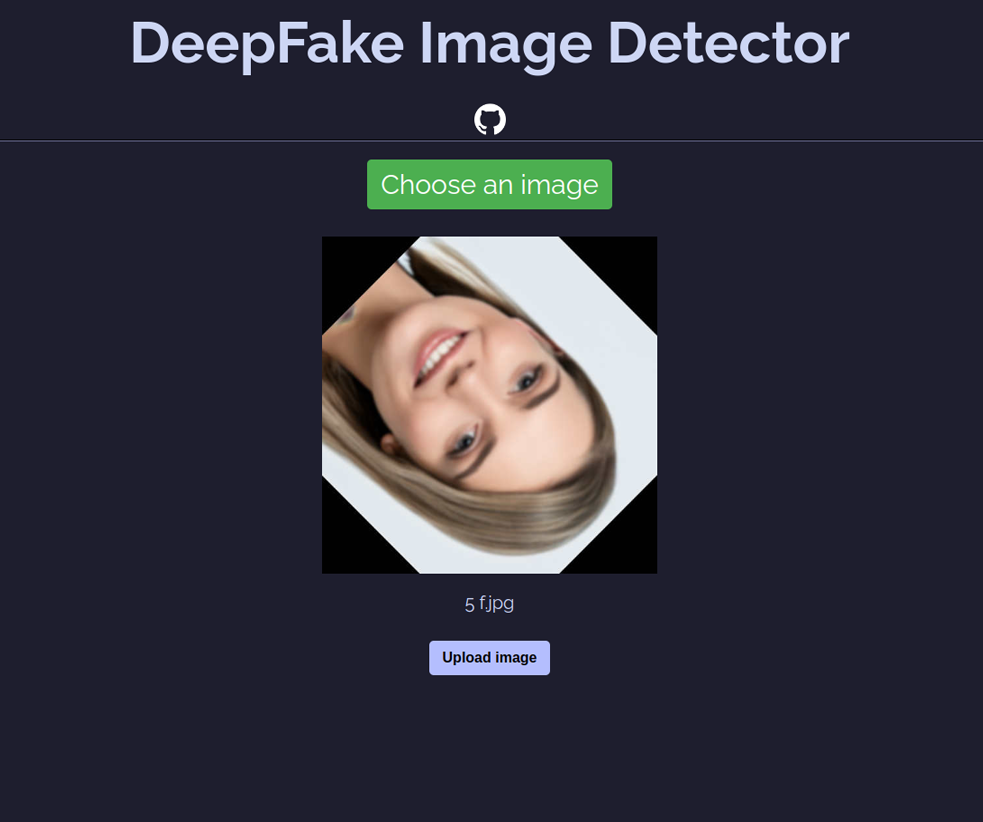
\includegraphics[width=0.66\textwidth]{./img/UI1.png}
		\caption{Preview Image}
	}
\end{figure}

\begin{figure}[hbt!]
	\center{
		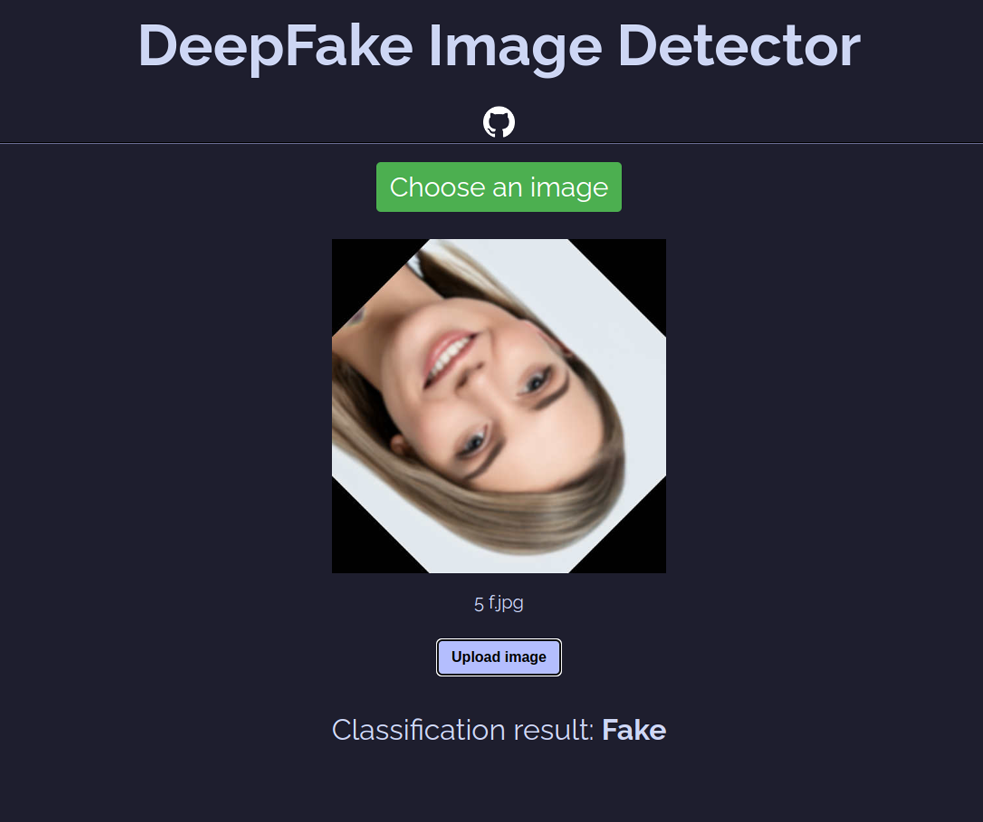
\includegraphics[width=0.66\textwidth]{./img/UI2.png}
		\caption{Demonstration of Model Classifying Image}
	}
\end{figure}